In this lab, an AC analysis of a common source amplifier with an NMOS transistor and a passive load is performed.
The circuit used for both sections of this lab is shown in figure \ref{fig:circuit}.

\FloatBarrier

\begin{figure}[h!]
	\centering
		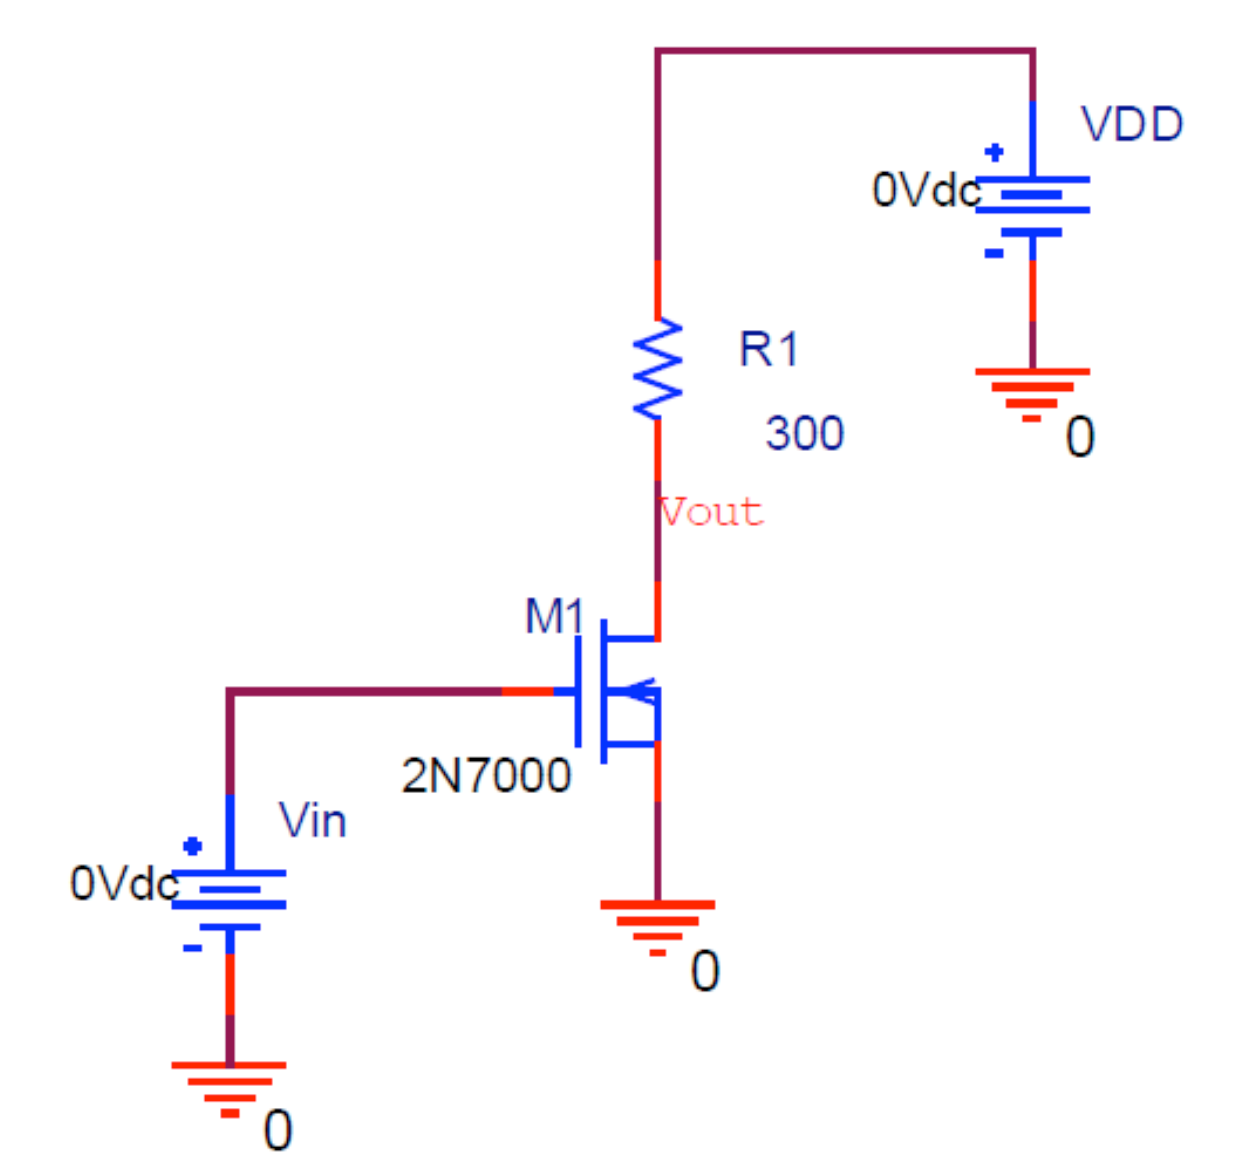
\includegraphics[scale=0.75]{./images/circuit.png}
			\caption{The Common Source NMOS Amplifier with a Passive Load}
			\label{fig:circuit}
			\end{figure}

\FloatBarrier

The voltage transfer characteristic is acquired. From the curve, the optimal bias point and threshold voltage are determined. The MOSFET's transconductance, amplifier bias current, and the gain of the amplifier are then acquired. They are compared to the theoretical values.
